\documentclass[xelatex,ja=standard,a4paper,14pt,everyparhook=compat]{bxjsarticle}
\usepackage{amsmath, amssymb, amsthm}
\usepackage{mathtools, bm}
\usepackage{graphicx, float}
\usepackage{hyperref}
\usepackage{enumerate}
% \usepackage{enumitem}
% \setenumerate{label=(\alph*)}
\usepackage{cancel}

% \usepackage{concmath}
% \usepackage[OT1]{fontenc}
\setsansfont{Segoe UI}
% \setmainfont{CMU Concrete}
% \usepackage{zxjatype}
\usepackage[noto-jp,oneweight]{zxjafont}
% \setCJKmainfont{Noto Serif JP}
% \setCJKsansfont{Noto Sans JP}

\usepackage{fancyhdr}
\pagestyle{fancy}
\lhead{\nouppercase{\leftmark}}
\rhead{\nouppercase{\rightmark}}
\renewcommand{\footrulewidth}{0.4pt}
\let\origtitle\title
\renewcommand{\title}[1]{\lfoot{#1}\origtitle{#1}}
\cfoot{}
\rfoot{\thepage}

\newcommand{\defby}{\overset{\mathrm{def}}{\iff}}

\newcommand{\bbC}{\mathbb{C}}
\newcommand{\bbR}{\mathbb{R}}
\newcommand{\bbQ}{\mathbb{Q}}
\newcommand{\bbZ}{\mathbb{Z}}
\newcommand{\bbN}{\mathbb{N}}
\newcommand{\bbP}{\mathbb{P}}
\newcommand{\bbF}{\mathbb{F}}
\newcommand{\mkS}{\mathfrak{S}}
\newcommand{\mkm}{\mathfrak{m}}
\newcommand{\mcA}{\mathcal{A}}
\newcommand{\mcB}{\mathcal{B}}
\newcommand{\mcC}{\mathcal{C}}
\newcommand{\mcH}{\mathcal{H}}
\newcommand{\mcL}{\mathcal{L}}
\newcommand{\mcS}{\mathcal{S}}
\newcommand{\umod}{{\bmod\:}}
\DeclareMathOperator{\inv}{inv}
\DeclareMathOperator{\conv}{conv}
\DeclareMathOperator{\image}{Im}
\DeclareMathOperator{\rank}{rank}
\DeclareMathOperator{\nullity}{null}
\DeclareMathOperator{\ess}{ess}
\DeclareMathOperator{\codim}{codim}

\theoremstyle{definition}
% \newtheorem{theorem}{定理}
\newtheorem*{theorem}{定理}
% \newtheorem{lemma}{補題}
\newtheorem*{lemma}{補題}
% \newtheorem{example}[theorem]{例}
\newtheorem*{example}{例}
% \newtheorem{definition}[theorem]{定義}
\newtheorem*{definition}{定義}
% \newtheorem{proposition}[theorem]{命題}
\newtheorem*{proposition}{命題}
% \newtheorem{corollary}[theorem]{系}
\newtheorem*{corollary}{系}
\newtheorem{problem}{問題}
\newtheorem*{answer}{解答}
\renewcommand{\proofname}{\textup{証明}}

\usepackage{tcolorbox}
\tcbuselibrary{breakable,skins,theorems}

\tcolorboxenvironment{definition}{
    coltitle = black,
    % colback = white,
    colframe = green!35!black,
    fonttitle = \bfseries,
    breakable = true
}

\tcolorboxenvironment{definition*}{
    coltitle = black,
    % colback = white,
    colframe = green!35!black,
    fonttitle = \bfseries,
    breakable = true
}

\tcolorboxenvironment{theorem}{
    coltitle = black,
    % colback = black!10!white,
    colframe = blue!35!black,
    fonttitle = \bfseries,
    breakable = true
}

\tcolorboxenvironment{theorem*}{
    coltitle = black,
    % colback = black!10!white,
    colframe = blue!35!black,
    fonttitle = \bfseries,
    breakable = true
}

\tcolorboxenvironment{proposition}{
    coltitle = black,
    % colback = black!10!white,
    colframe = blue!35!black,
    fonttitle = \bfseries,
    breakable = true
}

\tcolorboxenvironment{proposition*}{
    coltitle = black,
    % colback = black!10!white,
    colframe = blue!35!black,
    fonttitle = \bfseries,
    breakable = true
}

\tcolorboxenvironment{corollary}{
    coltitle = black,
    % colback = black!10!white,
    colframe = blue!35!black,
    fonttitle = \bfseries,
    breakable = true
}

\tcolorboxenvironment{corollary*}{
    coltitle = black,
    % colback = black!10!white,
    colframe = blue!35!black,
    fonttitle = \bfseries,
    breakable = true
}

\tcolorboxenvironment{lemma}{
    coltitle = black,
    % colback = black!10!white,
    colframe = green!35!black,
    fonttitle = \bfseries,
    breakable = true
}

\tcolorboxenvironment{example}{
    coltitle = black,
    colback = white,
    colframe = purple!35!black,
    fonttitle = \bfseries,
    breakable = true
}

\tcolorboxenvironment{example*}{
    coltitle = black,
    colback = white,
    colframe = purple!35!black,
    fonttitle = \bfseries,
    breakable = true
}

\tcolorboxenvironment{lemma*}{
    coltitle = black,
    % colback = black!10!white,
    colframe = gray!35!black,
    fonttitle = \bfseries,
    breakable = true
}

\tcolorboxenvironment{proof}{
    blanker,
    breakable,
    left=5mm,
    before skip=10pt,
    after skip=10pt,
    borderline west={1mm}{0pt}{black}
}

\tcolorboxenvironment{proof*}{
    blanker,
    breakable,
    left=5mm,
    before skip=10pt,
    after skip=10pt,
    borderline west={1mm}{0pt}{black}
}

\tcolorboxenvironment{problem}{
    coltitle = black,
    % colback = black!10!white,
    colframe = black!35!black,
    fonttitle = \bfseries,
    breakable = true
}

\tcolorboxenvironment{answer}{
    blanker,
    breakable,
    left=5mm,
    before skip=10pt,
    after skip=10pt,
    borderline west={1mm}{0pt}{black}
}

\title{3.20 Promotion and Evacuation}
\author{shino16}
\date{\today}

\begin{document}

\maketitle

\tableofcontents

\newpage

\setcounter{section}{-1}
\section{復習}

Poset $P$と$p = \#P$について,
\begin{align*}
    \bm p &= \text{$\{1,\ldots,p\}$に通常の順序がついたposet}, \\
    \mcL(P) &= (\text{$P$の線形拡大の集合}) \\
    &= \{f : \text{$P \to \bm p$, 大小関係を保つ全単射}\}
\end{align*}

$f(t)$は$t$のラベルと解釈できる.

\section{Promotion}

$f \in \mcL(P)$に以下の操作(promotion)を行って得られるものを$f\partial$とする:
\begin{enumerate}[1.]
    \item $f(t_1) = 1$なる$t_1$を取る.
    \item $t_2 = \operatorname{argmin} \{f(t_2) : t_1 \lessdot t_2\}$.
    \item $t_3 = \operatorname{argmin} \{f(t_3) : t_2 \lessdot t_3\}$.
    \item これを繰り返し,極大な元$t_k$を得るまで続ける.
    \item $f(t_1) \gets f(t_2)$,$f(t_2) \gets f(t_3)$,...,$f(t_{k-1}) \gets f(t_k)$と代入する.
    \item $f(t_k) \gets p+1$と代入し,全ての元のラベルを$1$減らす.
\end{enumerate}

$f\partial$は$f$の\textbf{promotion}.極大鎖$t_1 \lessdot t_2 \lessdot \cdots \lessdot t_k$は$f$の\textbf{promotion chain}.

\begin{figure}[H]
    \centering
    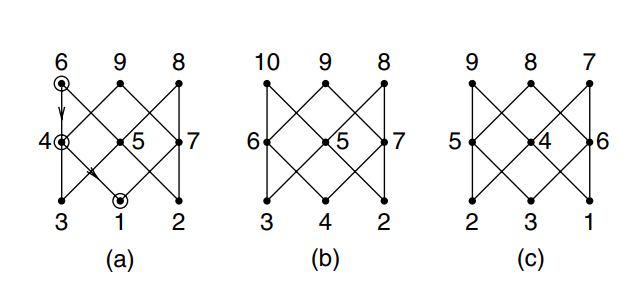
\includegraphics[width=.7\textwidth]{3.36.png}
    \caption{Promotion}
\end{figure}

$\delta$の双対な操作を\textbf{dual promotion} $\partial^*$とする.内容は:
\begin{enumerate}[1.]
    \item $f(t_1) = p$なる$t_1$を取る.
    \item $t_2 = \operatorname{argmax} \{f(t_2) : t_1 \gtrdot t_2\}$.
    \item $t_3 = \operatorname{argmax} \{f(t_3) : t_2 \gtrdot t_3\}$.
    \item これを繰り返し,極小な元$t_k$を得るまで続ける.
    \item $f(t_1) \gets f(t_2)$,$f(t_2) \gets f(t_3)$,...,$f(t_{k-1}) \gets f(t_k)$と代入する.
    \item $f(t_k) \gets 0$と代入し,全ての元のラベルを$1$増やす.
\end{enumerate}

$\partial^* = \partial^{-1}$に注意.

\newpage

$f \in \mcL(P)$に以下の操作(evacuation)を行って得られるものを$f\epsilon$とする.
\begin{enumerate}[1.]
    \item $f \gets f\partial$とし,ラベル$p$を固定する.
    \item $f$の残りのラベルのみに$\partial$を作用させ,さらにラベル$p-1$を固定する.
    \item $f$の残りのラベルのみに$\partial$を作用させ,さらにラベル$p-2$を固定する.
    \item これを$f$のラベルがすべて固定されるまで繰り返す.
\end{enumerate}

$f\epsilon$は$f$の\textbf{evacuation}.

\begin{figure}[ht]
    \centering
    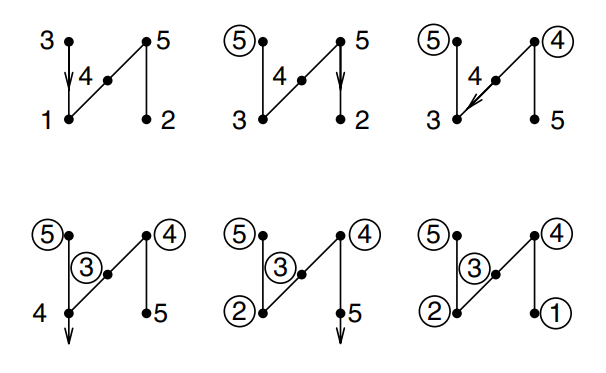
\includegraphics[width=.7\textwidth]{3.37.png}
    \caption{Evacuation}
\end{figure}

$\epsilon$の双対\textbf{dual evacuation} $\epsilon^*$も同様に定義する.つまり,ラベルを上に流して下方のラベルから固定していく.

\newpage

\begin{theorem}[3.20.1]
    \begin{enumerate}[(a)]
        \item $\epsilon^2 = 1$ (恒等写像).
        \item $\partial^p = \epsilon\epsilon^*$.
        \item $\partial\epsilon = \epsilon\partial^{-1}$.
    \end{enumerate}
\end{theorem}
この定理を示すのが3.20節の目標.

\begin{definition}
    \begin{align*}
        \text{群$G$} &= \langle \tau_1,\ldots,\tau_{p-1} \mid \text{$\tau_i^2 = 1$, $\tau_i \tau_j = \tau_j \tau_i$ if $|i-j| > 1$} \rangle, \\
        \delta_j &= \tau_1 \tau_2 \cdots \tau_j, \qquad (j=1,\ldots,p-1) \\
        \gamma_j &= \delta_j \delta_{j-1} \cdots \delta_1, \\
        \gamma^*_j &= (\tau_j \tau_{j-1} \cdots \tau_1)(\tau_j \tau_{j-1} \cdots \tau_2)\cdots(\tau_j \tau_{j-1}) (\tau_j).
    \end{align*}
\end{definition}

\begin{lemma}
    \begin{enumerate}[(a)]
        \item $\gamma_j^2 = (\gamma_j^*)^2 = 1$.
        \item $\delta_j^{j+1} = \gamma_j \gamma_j^*$.
        \item $\delta_j \gamma_j = \gamma_j \delta_j^{-1}$
    \end{enumerate}
\end{lemma}
\begin{proof}
    (a) $(\tau_1,\ldots,\tau_j)$を$(\tau_j,\ldots,\tau_1)$に置換すると$\gamma_j$は$\gamma_j^*$に変わる.よって$\gamma_j$についてのみ示せばよい.

    $j$の帰納法.$j=1$については \begin{align*}
        \gamma_1 &= \delta_1 = \tau_1, \\
        \tau_1^2 &= 1,
    \end{align*}
    よりOK.

    例えば \begin{align*}
        \gamma_4^2 &= (\tau_1 \tau_2 \tau_3 \tau_4) (\tau_1 \tau_2 \tau_3) (\tau_1 \cancel{\tau_2}) (\cancel{\tau_1}) (\cancel{\tau_1} \cancel{\tau_2} \tau_3 \tau_4) (\tau_1 \tau_2 \tau_3) (\tau_1 \tau_2) (\tau_1) \\
        &= (\tau_1 \tau_2 \tau_3 \tau_4) (\tau_1 \tau_2 \tau_3) \tau_1 (\tau_3 \tau_4) (\tau_1 \tau_2 \tau_3) (\tau_1 \tau_2) (\tau_1) \\
        &= (\tau_1 \tau_2 \tau_3) (\tau_1 \tau_2) \tau_1 \cancel{\tau_4} \cancel{\tau_3} (\cancel{\tau_3} \cancel{\tau_4}) (\tau_1 \tau_2 \tau_3) (\tau_1 \tau_2) (\tau_1) \\
        &= \gamma_3^2
    \end{align*}
    ということから,帰納的にOK.

    (b,c) $j$の帰納法で同様にやる.
\end{proof}

\begin{theorem}[3.20.1,再掲]
    \begin{enumerate}[(a)]
        \item $\epsilon^2 = 1$.
        \item $\partial^p = \epsilon\epsilon^*$.
        \item $\partial\epsilon = \epsilon\partial^{-1}$.
    \end{enumerate}
\end{theorem}

\begin{lemma}[再掲]
    \begin{enumerate}[(a)]
        \item $\gamma_j^2 = (\gamma_j^*)^2 = 1$.
        \item $\delta_j^{j+1} = \gamma_j \gamma_j^*$.
        \item $\delta_j \gamma_j = \gamma_j \delta_j^{-1}$
    \end{enumerate}
\end{lemma}

\begin{proof}[\textup{定理3.20.1の証明}]
    $f \in \mcL(P)$を$P$の元の列$u_1 u_2 \cdots u_p$と同一視する(ここで$f(u_i) = i$).

    $i=1,\ldots,p-1$について,$\tau_i : \mcL(P) \to \mcL(P)$を \begin{equation*}
        (u_1 u_2 \cdots u_p) \tau_i = \begin{cases*}
            u_1 u_2 \cdots u_i u_{i+1} \cdots u_p & if $u_i < u_{i+1}$, \\
            u_1 u_2 \cdots u_{i+1} u_i \cdots u_p & if $u_i$と$u_{i+1}$が比較不能,
        \end{cases*}
    \end{equation*}
    で定める.(なお$f(u_i) < f(u_{i+1})$より,$u_i > u_{i+1}$はあり得ない)

    あとは$\partial = \delta_{p-1}$と$\epsilon = \gamma_{p-1}$を示せば終わり.前者はお絵描き.後者はEvacuation $\epsilon$の定義と$\gamma_{p-1} = \delta_{p-1} \delta_{p-2} \cdots \delta_1$から.
\end{proof}

\end{document}
